\documentclass{article}
%\usepackage{authblk}
\usepackage{amssymb, amsmath}
\usepackage{hyperref}
\usepackage{verbatim}
\usepackage{multirow}
\usepackage{xcolor}
\usepackage{graphicx}
\usepackage{footnote}
\usepackage{array}
\usepackage{longtable}
\makesavenoteenv{tabular}

\addtolength{\hoffset}{-3.5cm}
\addtolength{\textwidth}{6.8cm}
\addtolength{\voffset}{-3cm}
\addtolength{\textheight}{6cm}

\newcommand{\NotImplementedYet}{\textbf{\color{orange}NI}}
\newcommand{\NotRanDueToDriverIssues}{\textbf{\color{orange}ND}}
\newcommand{\NotCorrect}{\textbf{\color{red}NC}}
\newcommand{\NotBuilding}{\textbf{\color{red}NB}}
\newcolumntype{P}[1]{>{\hspace{0pt}}p{#1}}


%\author[1]{Todor Milev}
%\affil[1]{FA Enterprise System}
\title{
Performance profiling \\
for FAB coin
}
\author{Todor Milev\footnote{FA Enterprise System}\\ todor@fa.biz}
\newcommand{\secpTwoFiveSixKone}{{\bf secp256k1}}
\renewcommand{\mod}{{~\bf mod~}}
\begin{document}
\maketitle
\section{Introduction}
In this text, we describe several performance profiling tests we carried out for FAB coin. 

In the present text, we focus on those performance characteristics that can be improved without changing the architecture of FAB coin.
%Not all performance characteristics of our system can be improved without modifying its architecture. 
The most important such characteristics are those of data management, networking and cryptography performance. Besides those, there are further performance characteristics that are not subject to immediate optimization without redesigning the system. For example, the average block mining time is 75 seconds by design: mining difficulty increases automatically to adjust for code improvements and network size increase. Those characteristics of the system are intimately tied to other properties such as the system's security and decentralization, and therefore cannot be improved by technical improvements of the code alone. We delegate further discussion of the architecture of FAB coin to other texts.


Our tests investigated the performance of individual FAB nodes on testNetNoDNS (an isolated self-contained tiny network), the performance of the tiny network testNetNoDNS as a whole, and finally the performance of individual nodes on mainNet. At the time of writing, testNetNoDNS has $3$ machines located on $3$ different continents. Should we decide it is worth the effort, we can deploy testNetNoDNS on more nodes; our setup can easily scale to an arbitrary number of machines.

Our preliminary tests show that - at least in our small testing environment - the data management and cryptography performance meets and significantly exceeds the current needs of a Fabcoin node. We do not expect that performance improvements in these two areas would significantly improve the speed of the whole system. However, we found that for the particular large memory pool transactions we tested, the network performance could be significantly improved. We have not yet investigated whether the performance limitations of the network were so by design (e.g., network traffic throttling) or were inadvertently caused by technical decisions in the fabcoind executable.

We plan on running our performance profiling system continuously to gather long term statistics and to hunt for performance regression bugs. Our performance profiling framework was designed to be expandable and maintainable, and we expect to add more statistics in the future. 

\subsection{Performance data gathered}
We profiled our network using two different scenarios. 

In the first scenario, we generated a large amount of transactions in the mempool on testNetNoDNS and tracked their propagation from the user interface to the local machine and from the local machine to the entire testNetNoDNS. More precisely, we generated one large transaction that split one input into $1000$ outputs, and then we generated 1000 small transactions, each transferring the output generated in the first transaction. In \eqref{eqThe1kTransaction}, the first transaction is denoted by $tx_0$ and the small transaction by $tx_{1},\dots, tx_{1000}$. All transactions were carried to and from one single address, and the initial coin source was a coinbase transaction.
\begin{equation}\label{eqThe1kTransaction}
25 \stackrel{tx_0}{\mapsto} \left\{\begin{array}{lcl}
0.025 & \stackrel{tx_1}{\mapsto}& 0.0245 \\
0.025 & \stackrel{tx_2}{\mapsto}& 0.0245\\
\vdots\\
0.025 & \stackrel{tx_{1000}}{\mapsto}& 0.0245
\end{array} \right.
\end{equation}
In the second scenario, we simply monitored the performance of individual non-mining nodes. Our mainNet nodes are non-user facing, so while they are compiled with wallet support, they did not perform any wallet actions.

\section{Setup}

We ran our tests on $3$ machines: a workstation in our local office in Markham, ON, Canada, and two AWS instances - one in London, UK and one in Mumbai, India. 

The ping times from the Canada machine to the London machine fluctuated about $200$ ms, with more than $1$ s for the first ping. The ping times from the Canada machine to the Mumbai machine fluctuated about $350$ ms, with more than $1$ s for the first ping. 

All machines ran our node.js server \url{https://github.com/blockchaingate/Kanban-js} as well as our modified fabcoind executable \url{https://github.com/tmilev/fabcoin} (our modifications amounted to more than 50 commits). 
\subsection{testNetNoDNS setup}
In order to carry out our experiments, we created a new fabcoind network, testNetNoDNS, while keeping the other three networks regtest, testNet and mainNet intact. On testNetNoDNS DNS peer discovery was disabled (similar to regtest and unlike testNet), however fixed-ip peers were pre-seeded (unlike regtest and similar to testNet). In this way, testNetNoDNS is an intermediate between regtest and testNet. We made a number of other modifications to testNetDNS to make our testing easier, including the following. 

\begin{itemize}
\item We changed the mining equihash parameters to $N=48$, $K=5$, allowing for sub-second mining of the first block. As the block mining difficulty takes time to adjust to the mining speed, we were able to mine the first $200$ blocks under a minute after each system reset.
\item We eased up the coinbase maturity restrictions: coinbase (coins obtained by mining) could be spend only after $100$ blocks.
\item We eased up the restrictions on memory pool chained transactions. Memory pool transactions that depend previous transactions that are still in the memory pool are restricted both by depth (number of linked transactions) and by byte size.
\end{itemize}

Many of the modified parameters were hard-coded in fabcoin (for example, the coinbase maturity constants); we refactored the fabcoind code as needed in order to keep the defaults for testNet and mainNet intact.

\subsection{Profiling code}
We profiled our code using a RAII (resource allocation is initialization) C++ technique which allowed us to track the performance of individual functions. The performance profiling was on an opt-in basis, achieved by adding a single line of code to the body of each profiled function. In this way, we were able to control the number of times our profiling code ran, ensuring our profiling does not slow down the system considerably. In the case of profiling that did not call other profiled functions, our profiling code incurred a time penalty of one mutex lock and one system clock call, which can safely be considered negligible when timing run times in the microseconds range. In the case of profiling nested functions, the profiling code run times were included in the statistics, worsening the reported performance of the outer functions. We have not yet investigated how significant is this effect. For simplicity, in the rest of this text we assume that the profiling code run times are negligible for all functions whose run times were in the milliseconds range. 

Nested function calls were accounted separately. Consider the following example.

\noindent\hfil\begin{minipage}{5cm}
\begin{verbatim}
void first()
{ 
  FunctionProfile profileThis("first");
  /* do useful work */  
}
void second()
{ 
  FunctionProfile profileThis("second");
  /* do useful work */  
  if (condition)
    first();
}
\end{verbatim}
\end{minipage}\hfil

In the code above, calling the function \verb|second| will cause the run time of \verb|second| and, when condition holds, the run time of \verb|second->first| to be recorded. At the same time, calling \verb|first| separately will cause the run time of \verb|first| to be directly recorded; here, we account \verb|second->first| and \verb|first| as different entries.

\subsection{Memory pool propagation speed}
Transaction arrival times to the memory pool were recorded the first time  \verb|AcceptToMemoryPoolWithTime| returned with \verb|true| for the given txid. All times were measured in POSIX time. We are assuming the clocks of all our machines are synchronized.

\section{Results}
\subsection{Memory pool propagation speed}
On the machine on which the transactions were submitted (located in Markham, Canada), the total run time of the routine \verb|AcceptToMemoryPool| for the $1001$ transactions given in \eqref{eqThe1kTransaction} fluctuated around $400$ milliseconds ($397$ milliseconds in our latest experiment). We find this speed to be satisfactory.

However, the speeds with which the transactions were received in our London and Mumbai machines were considerably worse. Tables \ref{tableArrivalTimesToLondon} and \ref{tableArrivalTimesToMumbai} show histograms of the arrival times - on the horizontal axis we have indicated the arrival delay in milliseconds (split into $50$ buckets of width about $1$ second each) and on the vertical axis we have indicated the number of txids that have arrived within the given time range.
\begin{table}
	\begin{center}
	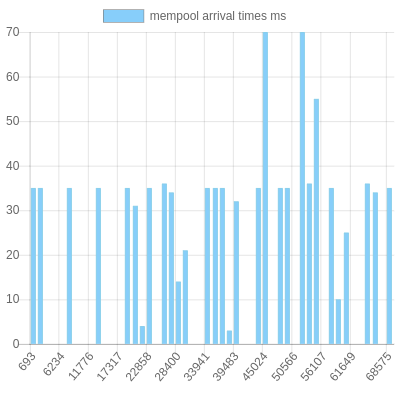
\includegraphics[width = 7cm]{./images/mempoolArrivalsLondon.png}
	\end{center}
	\caption{\label{tableArrivalTimesToLondon} Arrival delays in milliseconds Canada $ \to$ UK}
\end{table}

\begin{table}
	\begin{center}
		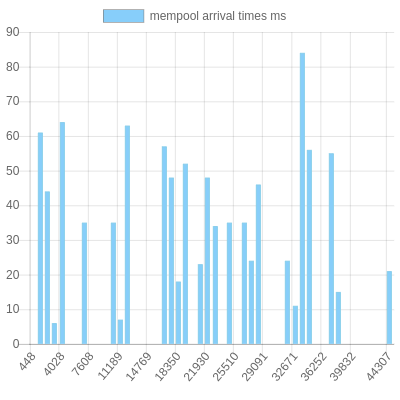
\includegraphics[width = 7cm]{./images/mempoolArrivalsMumbai.png}
	\end{center}
	\caption{\label{tableArrivalTimesToMumbai} Arrival delays in milliseconds Canada $ \to$ India}
\end{table}

For both machines, it took between $50$ and $60$ seconds for all transactions to arrive. Compared to about $400$ milliseconds needed for the transactions to be accepted to the first machine, this comprises a significant delay. The arrival times appear to be grouped into ``packets'' of size between $20$ to about $60$ transactions. It seems that this behavior is intentional and may be due to internal throttling of the network. Further investigation is required, however it is clear that with this performance we cannot propagate $1000$ transactions per second. Our conclusion here is that Kanban cannot rely on the fabcoin's networking stack ``out of the box'' as that was not designed to meet our performance goals. 


\subsection{Performance monitoring on testNetNoDNS}\label{secPerformanceMonitoringTestNetNoDNS}
In Table \ref{tablePerformanceLocalTestNetNoDNS}, we present the performance profile on testNetNoDNS on the machine that generated the $1001$ transactions. These statistics give us the best estimate of the performance of the memory pool in isolation of the network stack. More precisely, the function \verb|AcceptToMemoryPoolWithTime| gives us the best measure of the total running time of the database working in tandem with the cryptography stack and general transaction validation. On average, \verb|AcceptToMemoryPoolWithTime| takes $436$ microseconds to run, amounting to about more than 2200 transactions per second. It appears that this speed is satisfactory and exceeds the speed of the networking stack considerably. It also appears that this speed is sufficient to meet the current design goals of Kanban.  

We note that the performance of \verb|AcceptToMemoryPoolWithTime| on testNetNoDNS appears to be consistent with the performance on mainNet, however at the moment our mainNet sample is much smaller so we consider the data from testNetNoDNS to be a closer reflection of reality.

%We note that the database speeds appearing in our statistics on testNetNoDNS may be slightly better than what is expected on mainNet as the database on testNetNoDNS is very small.


\begin{table}
	Profiling recorded over 33 min, 34 s with 0 system restarts. Stats persist across restarts.
	
	\begin{longtable}{P{8cm}|r|r|r}
		Function&\# calls& Avg.run time $\mu$s& Run time excl. subord. \\\hline
		getmemorypoolarrivaltimes& 6& 2302&\\\hline
		sendBulkRawTransactions $\to$ sendOneRawTransaction $\to$ AcceptToMemoryPoolWithTime $\to$ AcceptToMemoryPoolWorker $\to$ VerifyScript& 2002& 75&\\\hline
		sendBulkRawTransactions $\to$ sendOneRawTransaction& 1001& 436&24\\\hline
		getperformanceprofile& 4& 10867&\\\hline
		sendBulkRawTransactions& 1& 444469&8464\\\hline
		dumpprivkey& 2& 47&\\\hline
		decoderawtransaction& 1& 155&\\\hline
		gettransaction& 1& 209&\\\hline
		getblockhash& 1& 10&\\\hline
		getbestblockhash& 1& 7&\\\hline
		sendBulkRawTransactions $\to$ sendOneRawTransaction $\to$ AcceptToMemoryPoolWithTime& 1001& 412&7\\\hline
		PeerLogicValidation :: ProcessMessages $\to$ ProcessMessage $\to$ ProcessHeadersMessage $\to$ UpdateBlockAvailability& 2& 3&\\\hline
		PeerLogicValidation :: ProcessMessages $\to$ ProcessMessage $\to$ ProcessHeadersMessage& 2& 27&24\\\hline
		PeerLogicValidation :: ProcessMessages $\to$ ProcessMessage $\to$ RelayAddress& 1& 12&\\\hline
		PeerLogicValidation :: ProcessMessages $\to$ ProcessGetData& 15& 94&\\\hline
		PeerLogicValidation :: ProcessMessages $\to$ ProcessMessage $\to$ ProcessGetData& 246& 288&\\\hline
		getnetworkinfo& 1& 76&\\\hline
		sendBulkRawTransactions $\to$ sendOneRawTransaction $\to$ AcceptToMemoryPoolWithTime $\to$ AcceptToMemoryPoolWorker& 1001& 405&255\\\hline
		getmininginfo& 8& 55&\\\hline
		getinfo& 2& 17223&\\\hline
		UpdateTip& 1& 116&\\\hline
		getmemoryinfo& 2& 336&\\\hline
		PeerLogicValidation :: SendMessages& 37117& 30&29\\\hline
		PeerLogicValidation :: UpdatedBlockTip& 1& 5&\\\hline
		PeerLogicValidation :: ProcessMessages $\to$ ProcessMessage& 341& 253&45\\\hline
		generatetoaddress& 2& 23712088&267294\\\hline
		PeerLogicValidation :: SendMessages $\to$ FindNextBlocksToDownload& 36910& 2&\\\hline
		PeerLogicValidation :: ProcessMessages& 37117& 6&3\\\hline
		generatetoaddress $\to$ Equihash :: BasicSolve& 84689& 553&\\\hline
		getpeerinfo& 2& 103&\\\hline
		LoadMempool& 1& 66&\\\hline
		listreceivedbyaddress& 3& 63&\\\hline
		generatetoaddress $\to$ UpdateTip& 210& 85&\\\hline
		getblock& 2& 196&\\\hline
		generatetoaddress $\to$ BlockAssembler :: CreateNewBlock& 210& 169&\\\hline
		generatetoaddress $\to$ PeerLogicValidation :: UpdatedBlockTip& 210& 7&\\\hline
	\end{longtable}

\caption{\label{tablePerformanceLocalTestNetNoDNS} Performance statistics, testNetNoDNS, local machine}
\end{table} 

\begin{table}
	
	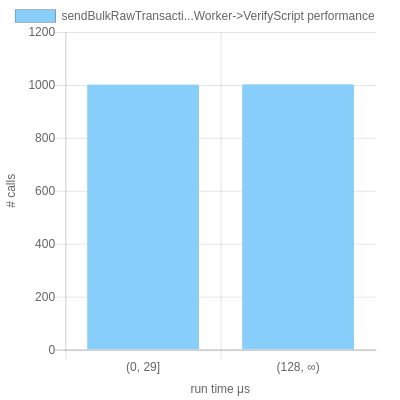
\includegraphics[width=7cm]{images/local/chartsendBulkRawTransactions-_3EsendOneRawTransaction-_3EAcceptToMemoryPoolWithTime-_3EAcceptToMemoryPoolWorker-_3EVerifyScript.png}
	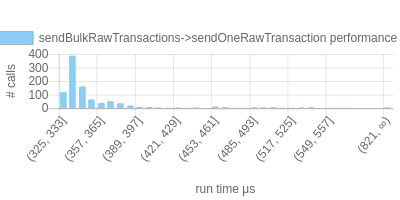
\includegraphics[width=7cm]{images/local/chartsendBulkRawTransactions-_3EsendOneRawTransaction.png}
	
	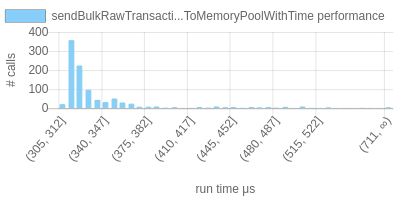
\includegraphics[width=7cm]{images/local/chartsendBulkRawTransactions-_3EsendOneRawTransaction-_3EAcceptToMemoryPoolWithTime.png}
	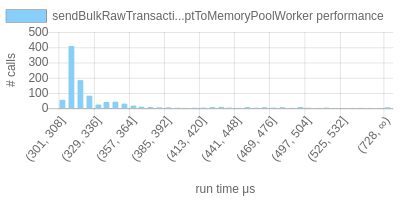
\includegraphics[width=7cm]{images/local/chartsendBulkRawTransactions-_3EsendOneRawTransaction-_3EAcceptToMemoryPoolWithTime-_3EAcceptToMemoryPoolWorker.png}
	
	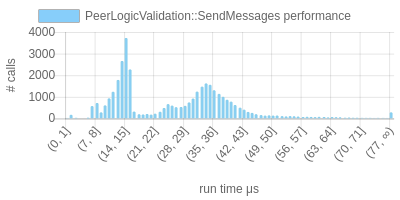
\includegraphics[width=7cm]{images/local/chartPeerLogicValidation_3A_3ASendMessages.png}
	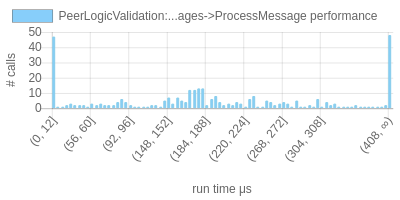
\includegraphics[width=7cm]{images/local/chartPeerLogicValidation_3A_3AProcessMessages-_3EProcessMessage.png}
	
	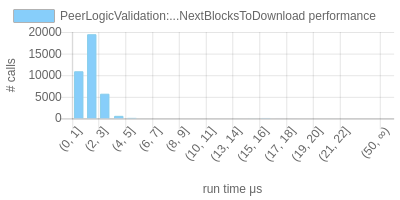
\includegraphics[width=7cm]{images/local/chartPeerLogicValidation_3A_3ASendMessages-_3EFindNextBlocksToDownload.png}
	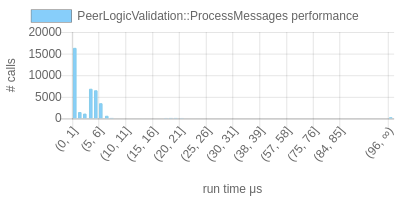
\includegraphics[width=7cm]{images/local/chartPeerLogicValidation_3A_3AProcessMessages.png}

	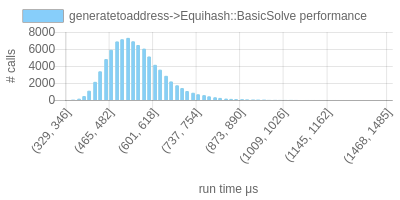
\includegraphics[width=7cm]{images/local/chartgeneratetoaddress-_3EEquihash_3A_3ABasicSolve.png}
	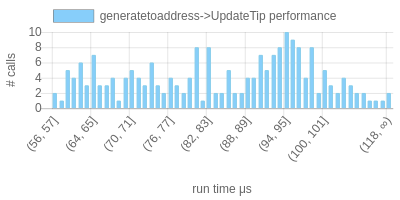
\includegraphics[width=7cm]{images/local/chartgeneratetoaddress-_3EUpdateTip.png}
	
	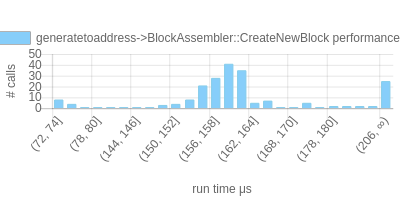
\includegraphics[width=7cm]{images/local/chartgeneratetoaddress-_3EBlockAssembler_3A_3ACreateNewBlock.png}
	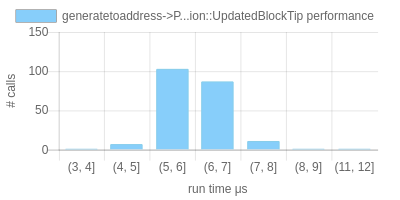
\includegraphics[width=7cm]{images/local/chartgeneratetoaddress-_3EPeerLogicValidation_3A_3AUpdatedBlockTip.png}
	
	
	\caption{Function run time histograms, testNetNoDNS, local machine}
\end{table}

\subsection{Performance monitoring on mainNet}
In the following tables, we present our results from monitoring mainNet over about 19 hours from our London and Mumbai machines. The first column of the two profiling tables shows the name of the function we profiled. Nesting of profiled functions is indicated by the $ \to $ arrow. The second column shows how many times did the function run over the course of our profiling. The third column shows the average run time of the function in microseconds. Please bear in mind that nested function calls incur a small performance penalty from the profiling code. For functions that call other profiled functions themselves, the fourth column indicates the run time of the function excluding the time of the profiled subroutines.


\subsubsection{Commentary}
Our statistics appear to show that the data management aspects - database access speeds and RAM memory management - are not a significant bottleneck for our system at the moment. For example, the \verb|UpdadeTip| function (executed when updating the leading block), takes 52 microseconds to run on average.

Our statistics also show that the cryptography stack is not a bottleneck either. For example the function \verb|VerifyScript|, which does the script verification and the cryptographic checks, has average run speed of about ranging from $160$ to about $180$ microseconds. This amounts to more than $5500$ transactions per second, which is two orders of magnitude large than the throughput of the network.


Our statistics also show that the cryptography stack and the database stack work in tandem together with a sufficient performance, confirming the observations from Section \ref{secPerformanceMonitoringTestNetNoDNS}.

Finally our statistics show that the networking stack has significant room for improvement. The network stack of fabcoin, in its present form, does meet the requirements of our Kanban project.



\subsubsection{Commentary on the right-corner spike of some graphs}
On both machines, the functions \verb|AcceptToMemoryPoolWorker| (and all of its callers) has a spike in run time that lies outside of the range of the histogram, causing all data to accumulate in the last bin of the histogram. 

Our histograms are centered as follows. First, we gather statistics without collecting histogram samples. Once we have averaged over a given number of runs (hand-coded for each function, defaults to $100$), we center our histogram using the average and choose the histogram so it has $50$ or less buckets on each side of the average. Evidently this strategy does not record well the performance of  \verb|AcceptToMemoryPoolWorker|; more work is required to gather more accurate statistics. Since this function has (on both the London and Mumbai machines) an average run time of some $6.5$ ms and is not called very frequently (several hundred times per day at the time of writing), investigating the matter does not appear to be of very high priority. 


The functions \verb|VerifyScript|, and to a lesser degree, \verb|SendMessages| showed similar out-of ordinary spikes in their histograms. The comments from the preceding paragraph apply to them as well; further investigation of the matter may be needed, but is not necessary in the short term.

\subsubsection{London machine}
Table  \ref{tablePerformanceLondon} shows the average running times of the profiled functions and Table \ref{graphsHistogramsLondon} shows their histograms.
\begin{table}
	Profiling recorded over 59 min, 15 s with 3 system restarts. Stats persist across restarts.
	
	\begin{longtable}{P{8cm}|r|r|r}
		Function&\# calls& Avg.run time $\mu$s& Run time excl. subord. \\\hline
		getmemorypoolarrivaltimes& 1& 7&\\\hline
		getmininginfo& 1& 43&\\\hline
		getinfo& 1& 90&\\\hline
		PeerLogicValidation :: ProcessMessages $\to$ ProcessMessage $\to$ AcceptToMemoryPoolWithTime $\to$ AcceptToMemoryPoolWorker $\to$ VerifyScript& 42& 70&\\\hline
		PeerLogicValidation :: ProcessMessages $\to$ ProcessMessage $\to$ AcceptToMemoryPoolWithTime $\to$ AcceptToMemoryPoolWorker& 11& 397&130\\\hline
		PeerLogicValidation :: ProcessMessages $\to$ ProcessMessage $\to$ AcceptToMemoryPoolWithTime& 11& 405&8\\\hline
		PeerLogicValidation :: ProcessMessages $\to$ ProcessMessage $\to$ ProcessMessage $\to$ PeerLogicValidation :: UpdatedBlockTip& 10& 4&\\\hline
		VerifyScript& 43702& 174&\\\hline
		PeerLogicValidation :: ProcessMessages $\to$ ProcessMessage $\to$ VerifyScript& 47942& 168&\\\hline
		getperformanceprofile& 11& 4263&\\\hline
		PeerLogicValidation :: ProcessMessages $\to$ ProcessMessage $\to$ RelayAddress& 2& 7&\\\hline
		LoadMempool& 3& 50&\\\hline
		getmemoryinfo& 9& 185&\\\hline
		UpdateTip& 6& 69&\\\hline
		PeerLogicValidation :: ProcessMessages $\to$ ProcessMessage $\to$ UpdateBlockAvailability& 202& 1&\\\hline
		PeerLogicValidation :: ProcessMessages& 404350& 1370&3\\\hline
		PeerLogicValidation :: ProcessMessages $\to$ ProcessMessage $\to$ ProcessHeadersMessage $\to$ UpdateBlockAvailability& 561& 2&\\\hline
		PeerLogicValidation :: ProcessMessages $\to$ ProcessMessage& 114239& 4838&3375\\\hline
		CDBIterator :: Next& 292442& 3&\\\hline
		PeerLogicValidation :: SendMessages $\to$ FindNextBlocksToDownload& 377284& 7&\\\hline
		PeerLogicValidation :: ProcessMessages $\to$ ProcessMessage $\to$ ProcessHeadersMessage& 561& 273734&273733\\\hline
		PeerLogicValidation :: SendMessages& 404349& 22&15\\\hline
		PeerLogicValidation :: UpdatedBlockTip& 6& 1&\\\hline
		PeerLogicValidation :: ProcessMessages $\to$ ProcessGetData& 15& 1386&\\\hline
		PeerLogicValidation :: ProcessMessages $\to$ ProcessMessage $\to$ PeerLogicValidation :: UpdatedBlockTip& 112796& 1&\\\hline
		PeerLogicValidation :: ProcessMessages $\to$ ProcessMessage $\to$ ProcessGetData& 88& 1440&\\\hline
		PeerLogicValidation :: ProcessMessages $\to$ ProcessMessage $\to$ UpdateTip& 112797& 47&\\\hline
		PeerLogicValidation :: ProcessMessages $\to$ ProcessMessage $\to$ ProcessMessage& 10& 1882&1738\\\hline
		PeerLogicValidation :: ProcessMessages $\to$ ProcessMessage $\to$ ProcessMessage $\to$ UpdateTip& 10& 140&\\\hline
	\end{longtable}
	\caption{\label{tablePerformanceLondon} Performance statistics mainNet, London machine}
\end{table}


\begin{table}
	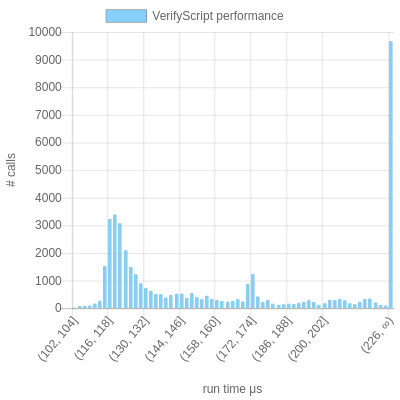
\includegraphics[width=7cm]{images/london/chartVerifyScript.png}
	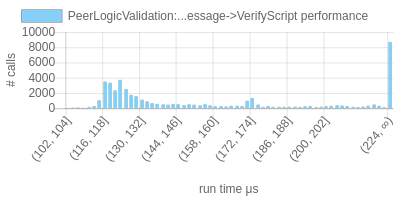
\includegraphics[width=7cm]{images/london/chartPeerLogicValidation_3A_3AProcessMessages-_3EProcessMessage-_3EVerifyScript.png}
	
	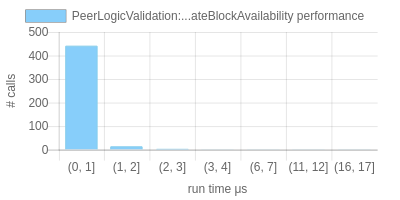
\includegraphics[width=7cm]{images/london/chartPeerLogicValidation_3A_3AProcessMessages-_3EProcessMessage-_3EUpdateBlockAvailability.png}
	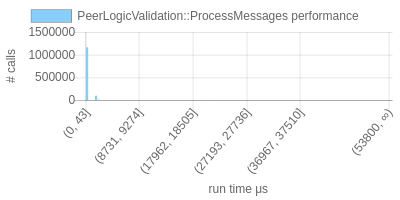
\includegraphics[width=7cm]{images/london/chartPeerLogicValidation_3A_3AProcessMessages.png}
	
	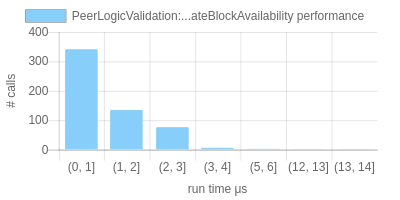
\includegraphics[width=7cm]{images/london/chartPeerLogicValidation_3A_3AProcessMessages-_3EProcessMessage-_3EProcessHeadersMessage-_3EUpdateBlockAvailability.png}
	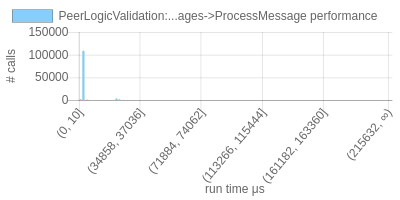
\includegraphics[width=7cm]{images/london/chartPeerLogicValidation_3A_3AProcessMessages-_3EProcessMessage.png}
	
	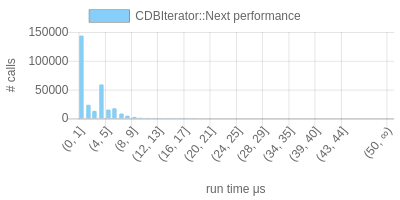
\includegraphics[width=7cm]{images/london/chartCDBIterator_3A_3ANext.png}
	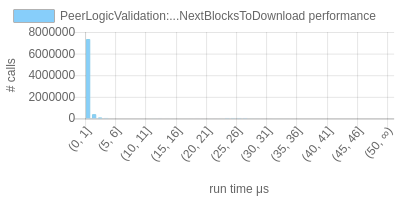
\includegraphics[width=7cm]{images/london/chartPeerLogicValidation_3A_3ASendMessages-_3EFindNextBlocksToDownload.png}
	
	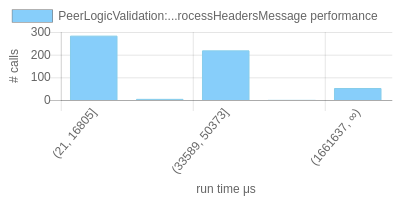
\includegraphics[width=7cm]{images/london/chartPeerLogicValidation_3A_3AProcessMessages-_3EProcessMessage-_3EProcessHeadersMessage.png}
	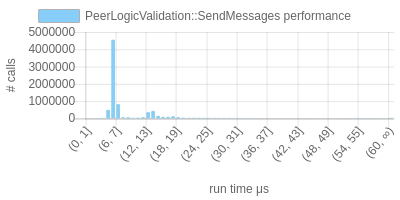
\includegraphics[width=7cm]{images/london/chartPeerLogicValidation_3A_3ASendMessages.png}
	
	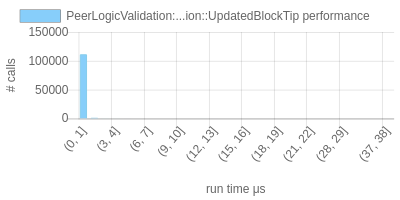
\includegraphics[width=7cm]{images/london/chartPeerLogicValidation_3A_3AProcessMessages-_3EProcessMessage-_3EPeerLogicValidation_3A_3AUpdatedBlockTip.png}
	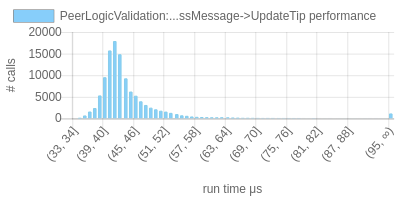
\includegraphics[width=7cm]{images/london/chartPeerLogicValidation_3A_3AProcessMessages-_3EProcessMessage-_3EUpdateTip.png}
	\caption{\label{graphsHistogramsLondon} Function run time histograms, mainNet, London machine}
\end{table}






\subsubsection{Mumbai machine}
Table  \ref{tablePerformanceMumbai} shows the average running times of the profiled functions and Table \ref{graphsHistogramsMumbai} shows their histograms.


\begin{table}
	Profiling recorded over 1 h, 2 min with 2 system restarts. Stats persist across restarts.
	
	\begin{longtable}{P{8cm}|r|r|r}
		Function&\# calls& Avg.run time $\mu$s& Run time excl. subord. \\\hline
		PeerLogicValidation :: ProcessMessages $\to$ ProcessMessage $\to$ AcceptToMemoryPoolWithTime $\to$ AcceptToMemoryPoolWorker $\to$ VerifyScript& 42& 73&\\\hline
		PeerLogicValidation :: ProcessMessages $\to$ ProcessMessage $\to$ AcceptToMemoryPoolWithTime $\to$ AcceptToMemoryPoolWorker& 11& 438&160\\\hline
		PeerLogicValidation :: ProcessMessages $\to$ ProcessMessage $\to$ AcceptToMemoryPoolWithTime& 11& 447&10\\\hline
		UpdateTip& 4& 87&\\\hline
		PeerLogicValidation :: ProcessMessages $\to$ ProcessMessage $\to$ UpdateBlockAvailability& 248& 2&\\\hline
		PeerLogicValidation :: ProcessMessages $\to$ ProcessMessage& 114906& 4773&3204\\\hline
		PeerLogicValidation :: ProcessMessages $\to$ ProcessMessage $\to$ ProcessMessage $\to$ PeerLogicValidation :: UpdatedBlockTip& 41& 5&\\\hline
		PeerLogicValidation :: ProcessMessages $\to$ ProcessMessage $\to$ RelayAddress& 11& 6&\\\hline
		CDBIterator :: Next& 192908& 3&\\\hline
		getperformanceprofile& 3& 3642&\\\hline
		PeerLogicValidation :: ProcessMessages $\to$ ProcessMessage $\to$ VerifyScript& 47696& 170&\\\hline
		VerifyScript& 43476& 177&\\\hline
		PeerLogicValidation :: ProcessMessages $\to$ ProcessMessage $\to$ ProcessHeadersMessage $\to$ UpdateBlockAvailability& 695& 2&\\\hline
		PeerLogicValidation :: ProcessMessages& 470499& 1169&3\\\hline
		PeerLogicValidation :: SendMessages $\to$ FindNextBlocksToDownload& 441304& 10&\\\hline
		PeerLogicValidation :: UpdatedBlockTip& 4& 2&\\\hline
		PeerLogicValidation :: ProcessMessages $\to$ ProcessMessage $\to$ ProcessHeadersMessage& 695& 238504&238502\\\hline
		PeerLogicValidation :: SendMessages& 470499& 25&15\\\hline
		getmemoryinfo& 6& 243&\\\hline
		LoadMempool& 3& 45&\\\hline
		PeerLogicValidation :: ProcessMessages $\to$ ProcessMessage $\to$ UpdateTip& 112602& 52&\\\hline
		PeerLogicValidation :: ProcessMessages $\to$ ProcessMessage $\to$ ProcessMessage& 41& 1985&1809\\\hline
		PeerLogicValidation :: ProcessMessages $\to$ ProcessMessage $\to$ ProcessMessage $\to$ UpdateTip& 41& 171&\\\hline
		PeerLogicValidation :: ProcessMessages $\to$ ProcessGetData& 15& 1380&\\\hline
		PeerLogicValidation :: ProcessMessages $\to$ ProcessMessage $\to$ PeerLogicValidation :: UpdatedBlockTip& 112601& 1&\\\hline
		PeerLogicValidation :: ProcessMessages $\to$ ProcessMessage $\to$ ProcessGetData& 306& 1062&\\\hline
	\end{longtable}
	\caption{\label{tablePerformanceMumbai} Performance statistics mainNet, Mumbai machine}
\end{table}

\begin{table}
	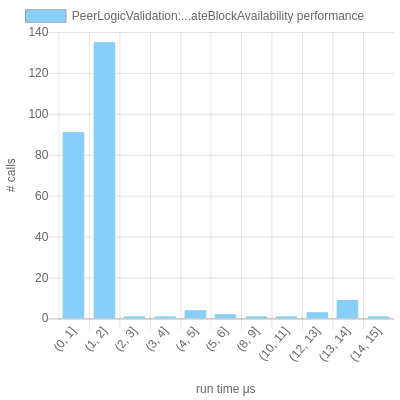
\includegraphics[width=7cm]{images/mumbai/chartPeerLogicValidation_3A_3AProcessMessages-_3EProcessMessage-_3EUpdateBlockAvailability.png}
	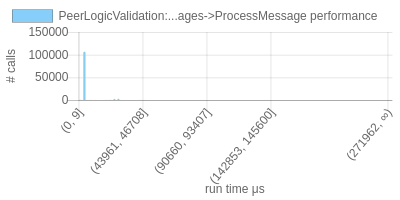
\includegraphics[width=7cm]{images/mumbai/chartPeerLogicValidation_3A_3AProcessMessages-_3EProcessMessage.png}
	
	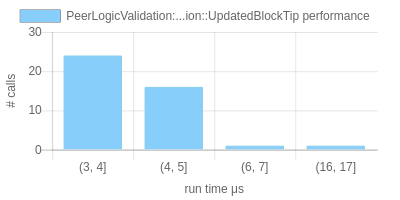
\includegraphics[width=7cm]{images/mumbai/chartPeerLogicValidation_3A_3AProcessMessages-_3EProcessMessage-_3EProcessMessage-_3EPeerLogicValidation_3A_3AUpdatedBlockTip.png}
	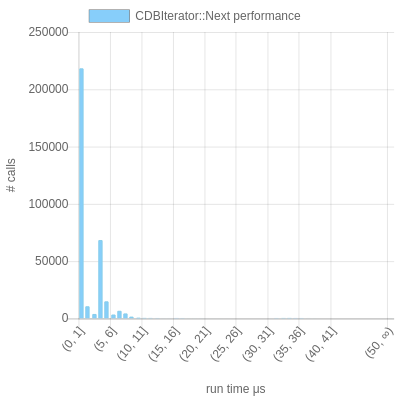
\includegraphics[width=7cm]{images/mumbai/chartCDBIterator_3A_3ANext.png}
	
	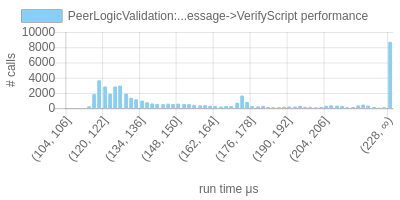
\includegraphics[width=7cm]{images/mumbai/chartPeerLogicValidation_3A_3AProcessMessages-_3EProcessMessage-_3EVerifyScript.png}
	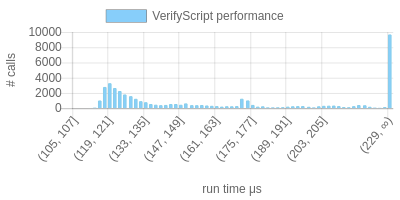
\includegraphics[width=7cm]{images/mumbai/chartVerifyScript.png}
	
	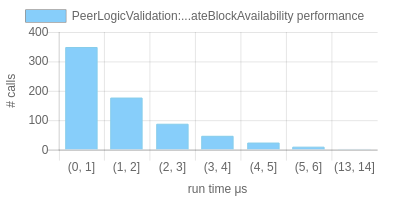
\includegraphics[width=7cm]{images/mumbai/chartPeerLogicValidation_3A_3AProcessMessages-_3EProcessMessage-_3EProcessHeadersMessage-_3EUpdateBlockAvailability.png}
	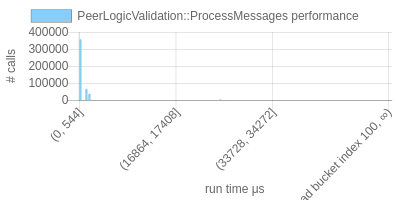
\includegraphics[width=7cm]{images/mumbai/chartPeerLogicValidation_3A_3AProcessMessages.png}
	
	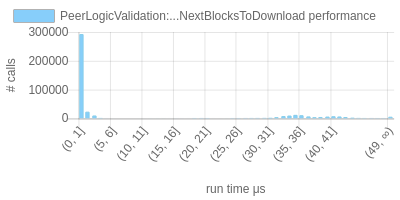
\includegraphics[width=7cm]{images/mumbai/chartPeerLogicValidation_3A_3ASendMessages-_3EFindNextBlocksToDownload.png}
	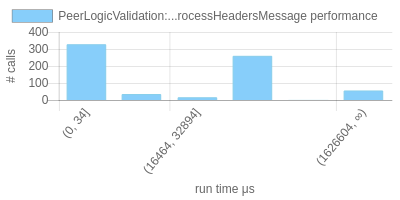
\includegraphics[width=7cm]{images/mumbai/chartPeerLogicValidation_3A_3AProcessMessages-_3EProcessMessage-_3EProcessHeadersMessage.png}
	
	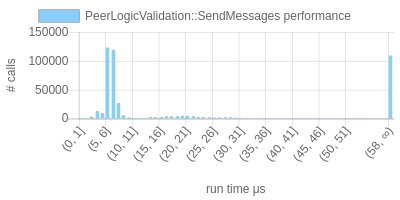
\includegraphics[width=5cm]{images/mumbai/chartPeerLogicValidation_3A_3ASendMessages.png}
	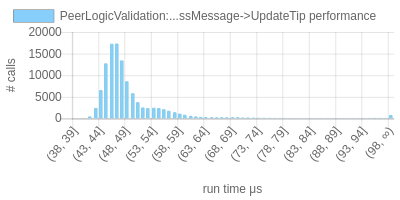
\includegraphics[width=5cm]{images/mumbai/chartPeerLogicValidation_3A_3AProcessMessages-_3EProcessMessage-_3EUpdateTip.png}	
	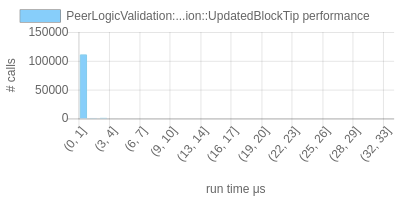
\includegraphics[width=5cm]{images/mumbai/chartPeerLogicValidation_3A_3AProcessMessages-_3EProcessMessage-_3EPeerLogicValidation_3A_3AUpdatedBlockTip.png}
	\caption{\label{graphsHistogramsMumbai} Function run time histograms, mainNet, Mumbai machine}
\end{table}

\bibliographystyle{plain}
\bibliography{../bibliography}
\end{document}
